\documentclass{standalone}
\usepackage{tikz}
\usetikzlibrary{patterns, positioning}
\usepackage[sfdefault]{ClearSans} %% option 'sfdefault' activates Clear Sans as the default text font
\usepackage[T1]{fontenc}

\begin{document}
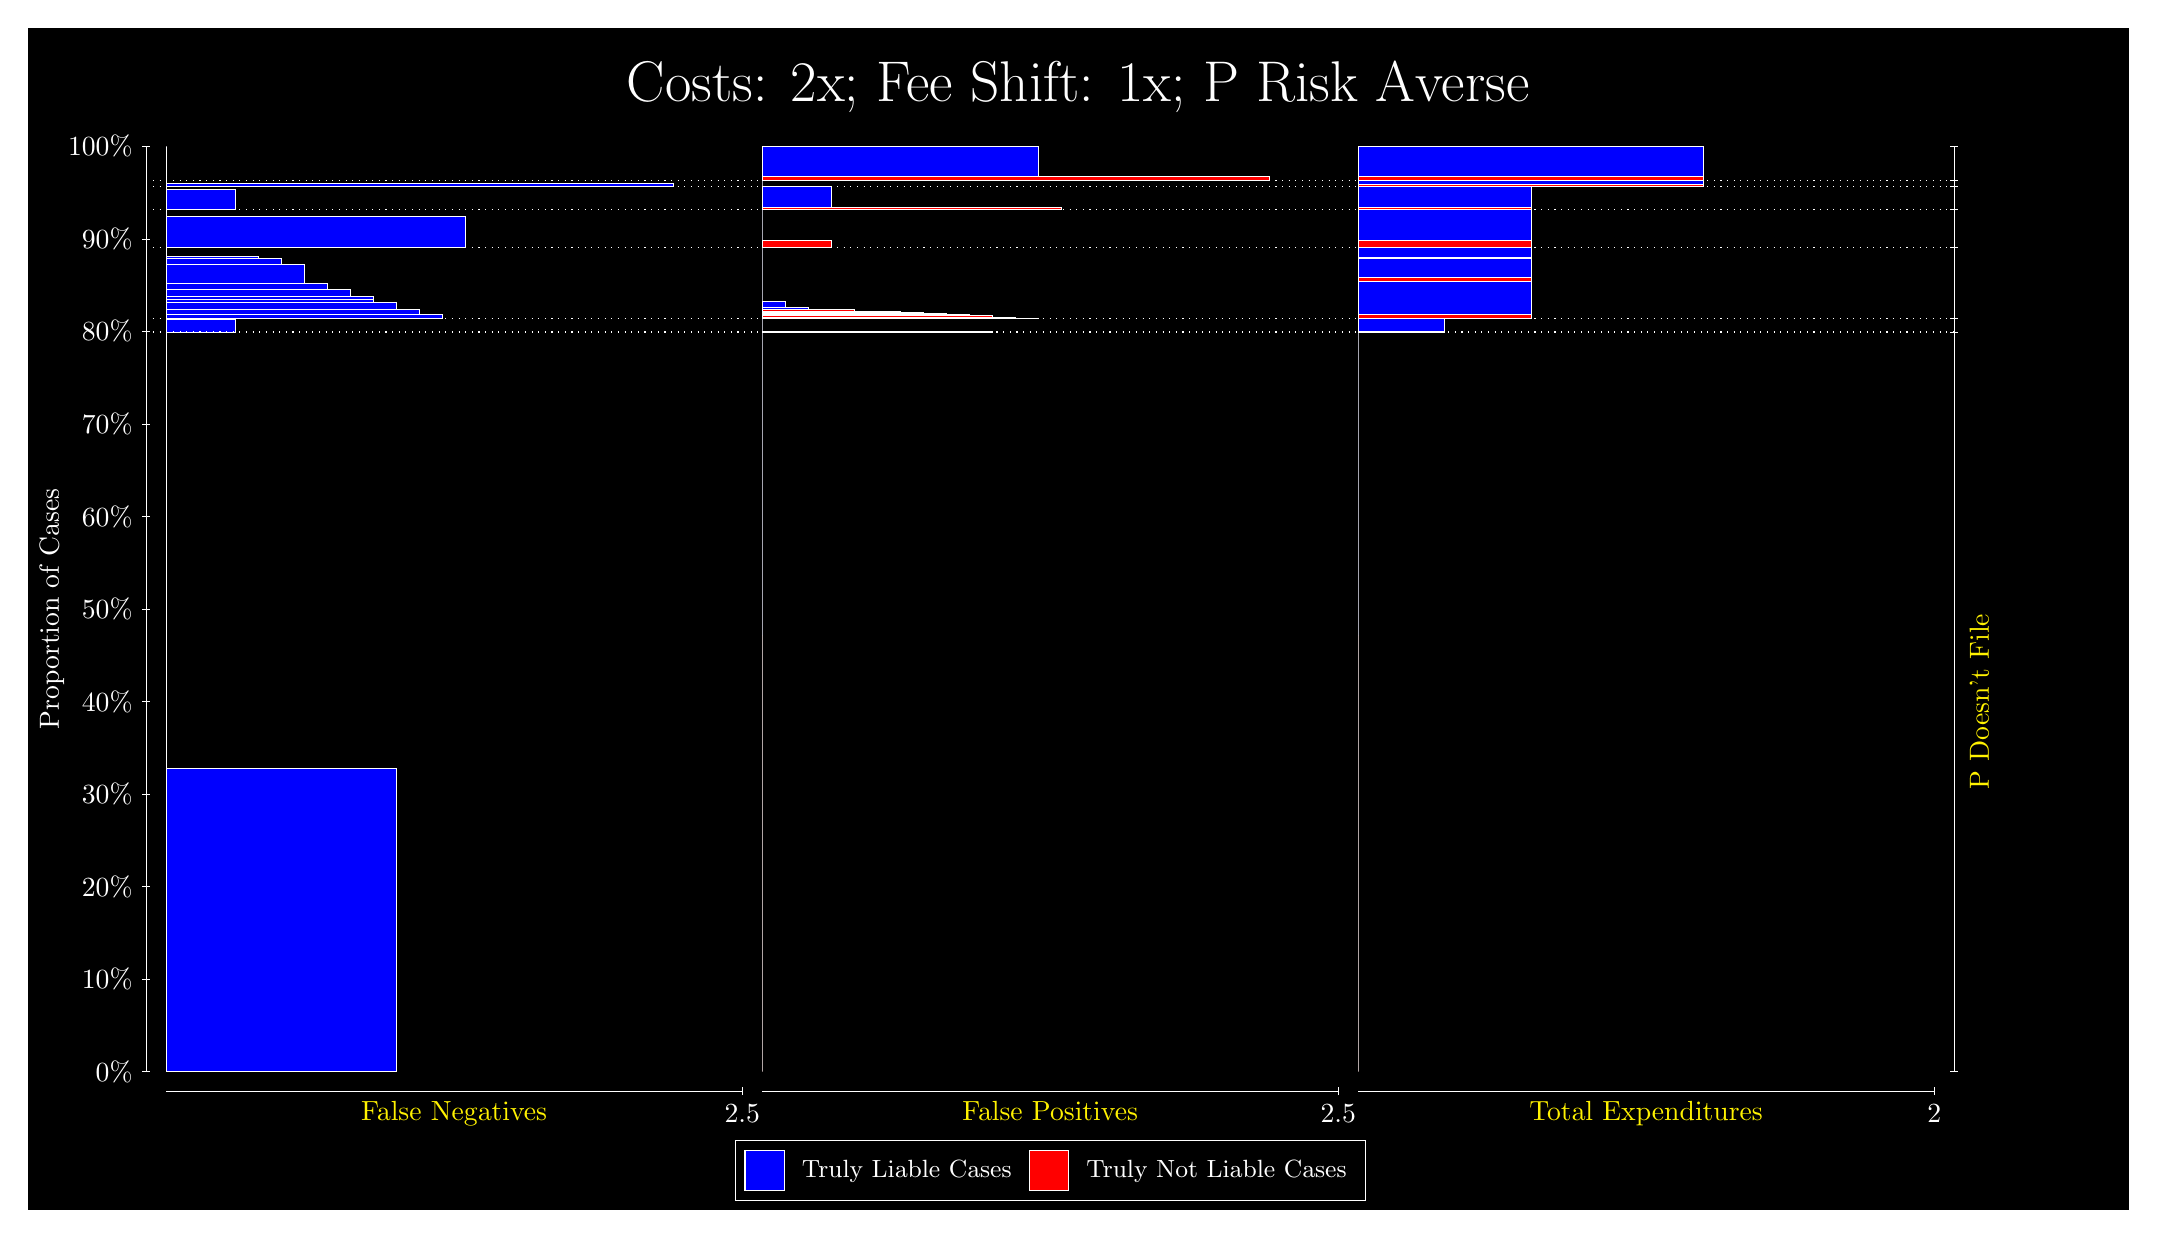
\begin{tikzpicture}
\draw[fill=black] (0,0) rectangle (26.667,15);
\draw[text=white] (0,13.5) rectangle (26.667,15) node[midway] {\huge Costs: 2x; Fee Shift: 1x; P Risk Averse};
\draw[white, very thin] (1.5,1.75) -- (1.5,13.5);
\node[rotate=90, text=white, anchor=center] at (0.3, 7.625) {Proportion of Cases};
\draw[white, very thin] (1.45,1.75) -- (1.55,1.75);
\node[text=white, anchor=east] at (1.45, 1.75) {0\%};
\draw[white, very thin] (1.45,2.925) -- (1.55,2.925);
\node[text=white, anchor=east] at (1.45, 2.925) {10\%};
\draw[white, very thin] (1.45,4.1) -- (1.55,4.1);
\node[text=white, anchor=east] at (1.45, 4.1) {20\%};
\draw[white, very thin] (1.45,5.275) -- (1.55,5.275);
\node[text=white, anchor=east] at (1.45, 5.275) {30\%};
\draw[white, very thin] (1.45,6.45) -- (1.55,6.45);
\node[text=white, anchor=east] at (1.45, 6.45) {40\%};
\draw[white, very thin] (1.45,7.625) -- (1.55,7.625);
\node[text=white, anchor=east] at (1.45, 7.625) {50\%};
\draw[white, very thin] (1.45,8.8) -- (1.55,8.8);
\node[text=white, anchor=east] at (1.45, 8.8) {60\%};
\draw[white, very thin] (1.45,9.975) -- (1.55,9.975);
\node[text=white, anchor=east] at (1.45, 9.975) {70\%};
\draw[white, very thin] (1.45,11.15) -- (1.55,11.15);
\node[text=white, anchor=east] at (1.45, 11.15) {80\%};
\draw[white, very thin] (1.45,12.325) -- (1.55,12.325);
\node[text=white, anchor=east] at (1.45, 12.325) {90\%};
\draw[white, very thin] (1.45,13.5) -- (1.55,13.5);
\node[text=white, anchor=east] at (1.45, 13.5) {100\%};

\draw[white, very thin] (24.457,1.75) -- (24.457,13.5);
\draw[white, very thin] (24.407,1.75) -- (24.507,1.75);
\node[anchor=west] at (24.407, 1.75) {};
\draw[white, very thin] (24.407,11.142) -- (24.507,11.142);
\node[anchor=west] at (24.407, 11.142) {};
\draw[white, very thin] (24.407,11.319) -- (24.507,11.319);
\node[anchor=west] at (24.407, 11.319) {};
\draw[white, very thin] (24.407,12.217) -- (24.507,12.217);
\node[anchor=west] at (24.407, 12.217) {};
\draw[white, very thin] (24.407,12.7) -- (24.507,12.7);
\node[anchor=west] at (24.407, 12.7) {};
\draw[white, very thin] (24.407,12.988) -- (24.507,12.988);
\node[anchor=west] at (24.407, 12.988) {};
\draw[white, very thin] (24.407,13.07) -- (24.507,13.07);
\node[anchor=west] at (24.407, 13.07) {};
\draw[white, very thin] (24.407,13.5) -- (24.507,13.5);
\node[anchor=west] at (24.407, 13.5) {};

\draw[white, very thin, fill=blue] (1.75,1.75) rectangle (4.6775,5.5991);
\draw[white, very thin, fill=red] (1.75,5.5991) rectangle (1.75,11.142);
\draw[white, very thin, fill=blue] (1.75,11.142) rectangle (2.6283,11.306);
\draw[white, very thin, fill=red] (1.75,11.306) rectangle (1.75,11.319);
\draw[white, very thin, fill=blue] (1.75,11.319) rectangle (5.2631,11.371);
\draw[white, very thin, fill=blue] (1.75,11.371) rectangle (4.9703,11.425);
\draw[white, very thin, fill=blue] (1.75,11.425) rectangle (4.6775,11.516);
\draw[white, very thin, fill=blue] (1.75,11.516) rectangle (4.3848,11.561);
\draw[white, very thin, fill=blue] (1.75,11.561) rectangle (4.3848,11.59);
\draw[white, very thin, fill=blue] (1.75,11.59) rectangle (4.092,11.688);
\draw[white, very thin, fill=blue] (1.75,11.688) rectangle (3.7993,11.759);
\draw[white, very thin, fill=blue] (1.75,11.759) rectangle (3.5065,12.002);
\draw[white, very thin, fill=blue] (1.75,12.002) rectangle (3.2138,12.079);
\draw[white, very thin, fill=blue] (1.75,12.079) rectangle (2.921,12.106);
\draw[white, very thin, fill=red] (1.75,12.106) rectangle (1.75,12.217);
\draw[white, very thin, fill=blue] (1.75,12.217) rectangle (5.5558,12.607);
\draw[white, very thin, fill=red] (1.75,12.607) rectangle (1.75,12.7);
\draw[white, very thin, fill=blue] (1.75,12.7) rectangle (2.6283,12.958);
\draw[white, very thin, fill=red] (1.75,12.958) rectangle (1.75,12.988);
\draw[white, very thin, fill=blue] (1.75,12.988) rectangle (8.1906,13.037);
\draw[white, very thin, fill=red] (1.75,13.037) rectangle (1.75,13.07);
\draw[white, very thin, fill=red] (1.75,13.07) rectangle (1.75,13.121);
\draw[white, very thin, fill=blue] (1.75,13.121) rectangle (1.75,13.5);
\draw[white, very thin, fill=red] (9.3189,1.75) rectangle (9.3189,7.2932);
\draw[white, very thin, fill=blue] (9.3189,7.2932) rectangle (9.3189,11.142);
\draw[white, very thin, fill=red] (9.3189,11.142) rectangle (12.246,11.156);
\draw[white, very thin, fill=blue] (9.3189,11.156) rectangle (9.3189,11.319);
\draw[white, very thin, fill=red] (9.3189,11.319) rectangle (12.832,11.322);
\draw[white, very thin, fill=red] (9.3189,11.322) rectangle (12.539,11.331);
\draw[white, very thin, fill=red] (9.3189,11.331) rectangle (12.246,11.355);
\draw[white, very thin, fill=red] (9.3189,11.355) rectangle (11.954,11.364);
\draw[white, very thin, fill=red] (9.3189,11.364) rectangle (11.661,11.378);
\draw[white, very thin, fill=red] (9.3189,11.378) rectangle (11.368,11.387);
\draw[white, very thin, fill=red] (9.3189,11.387) rectangle (11.075,11.402);
\draw[white, very thin, fill=red] (9.3189,11.402) rectangle (10.783,11.41);
\draw[white, very thin, fill=red] (9.3189,11.41) rectangle (10.49,11.431);
\draw[white, very thin, fill=blue] (9.3189,11.431) rectangle (9.9044,11.457);
\draw[white, very thin, fill=blue] (9.3189,11.457) rectangle (9.6116,11.534);
\draw[white, very thin, fill=blue] (9.3189,11.534) rectangle (9.3189,12.217);
\draw[white, very thin, fill=red] (9.3189,12.217) rectangle (10.197,12.311);
\draw[white, very thin, fill=blue] (9.3189,12.311) rectangle (9.3189,12.7);
\draw[white, very thin, fill=red] (9.3189,12.7) rectangle (13.125,12.73);
\draw[white, very thin, fill=blue] (9.3189,12.73) rectangle (10.197,12.988);
\draw[white, very thin, fill=red] (9.3189,12.988) rectangle (9.3189,13.02);
\draw[white, very thin, fill=blue] (9.3189,13.02) rectangle (9.3189,13.07);
\draw[white, very thin, fill=red] (9.3189,13.07) rectangle (15.759,13.121);
\draw[white, very thin, fill=blue] (9.3189,13.121) rectangle (12.832,13.5);
\draw[white, very thin, fill=red] (16.888,1.75) rectangle (16.888,7.2932);
\draw[white, very thin, fill=blue] (16.888,7.2932) rectangle (16.888,11.142);
\draw[white, very thin, fill=red] (16.888,11.142) rectangle (17.986,11.156);
\draw[white, very thin, fill=blue] (16.888,11.156) rectangle (17.986,11.319);
\draw[white, very thin, fill=red] (16.888,11.319) rectangle (19.083,11.365);
\draw[white, very thin, fill=blue] (16.888,11.365) rectangle (19.083,11.783);
\draw[white, very thin, fill=red] (16.888,11.783) rectangle (19.083,11.832);
\draw[white, very thin, fill=blue] (16.888,11.832) rectangle (19.083,12.074);
\draw[white, very thin, fill=red] (16.888,12.074) rectangle (19.083,12.091);
\draw[white, very thin, fill=blue] (16.888,12.091) rectangle (19.083,12.217);
\draw[white, very thin, fill=red] (16.888,12.217) rectangle (19.083,12.311);
\draw[white, very thin, fill=blue] (16.888,12.311) rectangle (19.083,12.7);
\draw[white, very thin, fill=red] (16.888,12.7) rectangle (19.083,12.73);
\draw[white, very thin, fill=blue] (16.888,12.73) rectangle (19.083,12.988);
\draw[white, very thin, fill=red] (16.888,12.988) rectangle (21.279,13.02);
\draw[white, very thin, fill=blue] (16.888,13.02) rectangle (21.279,13.07);
\draw[white, very thin, fill=red] (16.888,13.07) rectangle (21.279,13.121);
\draw[white, very thin, fill=blue] (16.888,13.121) rectangle (21.279,13.5);
\draw[white, dotted] (1.5,11.142) -- (24.457,11.142);
\draw[white, dotted] (1.5,11.319) -- (24.457,11.319);
\draw[white, dotted] (1.5,12.217) -- (24.457,12.217);
\draw[white, dotted] (1.5,12.7) -- (24.457,12.7);
\draw[white, dotted] (1.5,12.988) -- (24.457,12.988);
\draw[white, dotted] (1.5,13.07) -- (24.457,13.07);
\draw[white, very thin] (1.75,1.5) -- (9.0689,1.5);
\node[text=yellow, anchor=north] at (5.4094, 1.5) {False Negatives};
\draw[white, very thin] (9.0689,1.45) -- (9.0689,1.55);
\node[text=white, anchor=north] at (9.0689, 1.45) {2.5};

\draw[white, very thin] (9.3189,1.5) -- (16.638,1.5);
\node[text=yellow, anchor=north] at (12.978, 1.5) {False Positives};
\draw[white, very thin] (16.638,1.45) -- (16.638,1.55);
\node[text=white, anchor=north] at (16.638, 1.45) {2.5};

\draw[white, very thin] (16.888,1.5) -- (24.207,1.5);
\node[text=yellow, anchor=north] at (20.547, 1.5) {Total Expenditures};
\draw[white, very thin] (24.207,1.45) -- (24.207,1.55);
\node[text=white, anchor=north] at (24.207, 1.45) {2};

\node[text=yellow, centered, rotate=90] at (24.777, 6.4462) {P Doesn't File};







\draw (12.978300999999998,1.5) node[draw=none] (baseCoordinate) {};
\begin{scope}[align=center]
        \matrix[scale=0.5, draw=white, below=0.5cm of baseCoordinate, nodes={draw}, column sep=0.1cm]{
            \node[rectangle, draw, minimum width=0.5cm, minimum height=0.5cm, fill=blue] {}; &
            \node[draw=none, font=\small, text=white] (B) {Truly Liable Cases}; &
            \node[rectangle, draw, minimum width=0.5cm, minimum height=0.5cm, fill=red] {}; &
            \node[draw=none, font=\small, text=white] (B) {Truly Not Liable Cases}; \\
            };
\end{scope}

\end{tikzpicture}
\end{document}